\section{Propósito del proyecto}

\subsection{Contexto}

La aplicación se enmarca en el contexto de la gestión de recursos en el ámbito
empresarial. En este caso, la aplicación no tiene un objetivo comercial, será
usada solamente por los empleados de Ingeniería e Innovación.

\subsection{Objetivo general}

El objetivo es desarrollar una herramienta de fácil uso para que los empleados
de Ingeniería e Innovación puedan llevar un registro detallado de los recursos
humanos empleados en los proyectos que gestionan.

\section{El cliente y otros interesados}

\subsection{El cliente}

El único cliente es Ingeniería e Innovación.

\subsection{Otros interesados}

\begin{itemize}
 \item Desarrollador: en este caso, el proyectante, Javier Cejudo, se encarga
de todos los aspectos relacionados con el desarrollo del sistema desde sus
primeras etapas hasta la finalización del mismo.

\item Tutor: Ángel Luis Rubio, se encarga de la orientación del proyecto para
que se adecue a lo que debe ser un PFC.

\item Tutor de empresa: León Arnedo, es en cierto modo el principal
representante del cliente, pero también se encarga de la orientación del
proyecto para que se adecue a sus necesidades.
Es también el principal \textit{testeador} de la aplicación.
\end{itemize}


\section{Los usuarios del producto}

\subsection{Usuarios finales}

\begin{itemize}
 \item Los empleados de la empresa: todos tienen amplia
experiencia en el uso de sistemas de información. De hecho, la herramienta a
desarrollar en este proyecto se integrará en una intranet de uso común a todos
los empleados.

\item Usuarios de mantenimiento: el mantenimiento será llevado a cabo por
alguno de los empleados de la empresa con conocimientos de PHP. Todos son
ingenieros industriales sin amplia experiencia en el tema.
\end{itemize}

\subsection{Prioridades asignadas a los usuarios}

Por la naturaleza del sistema, y ya que no se prevé que vayan a
ser necesarias ampliaciones considerables, los usuarios finales serán la
prioridad a la hora de diseñar el producto; los usuarios de mantenimiento se
encargarían de solucionar problemas potenciales o realizar cambios mínimos.

\section{Tecnologías a utilizar}
\label{sec:tecnologias}

La decisión acerca de las tecnologías a utilizar se ha basado casi
exclusivamente en los requisitos de Ingeniería e Innovación. La arquitectura
básica de la aplicación (la de la empresa puede verse en la figura
\ref{fig:arquitectura_iandi}) consiste en un servidor ejecutando sobre Microsoft
Windows con una base de datos MySQL interpretada en el lado del servidor
mediante PHP, cuyo código resultante es gestionado por el servidor web HTTP
Apache. La nueva funcionalidad que proporciona el desarrollo de este proyecto
debía integrarse de forma consistente, de manera que esas serán las tecnologías
que soporten el desarrollo del proyecto.

\begin{figure}
\centering
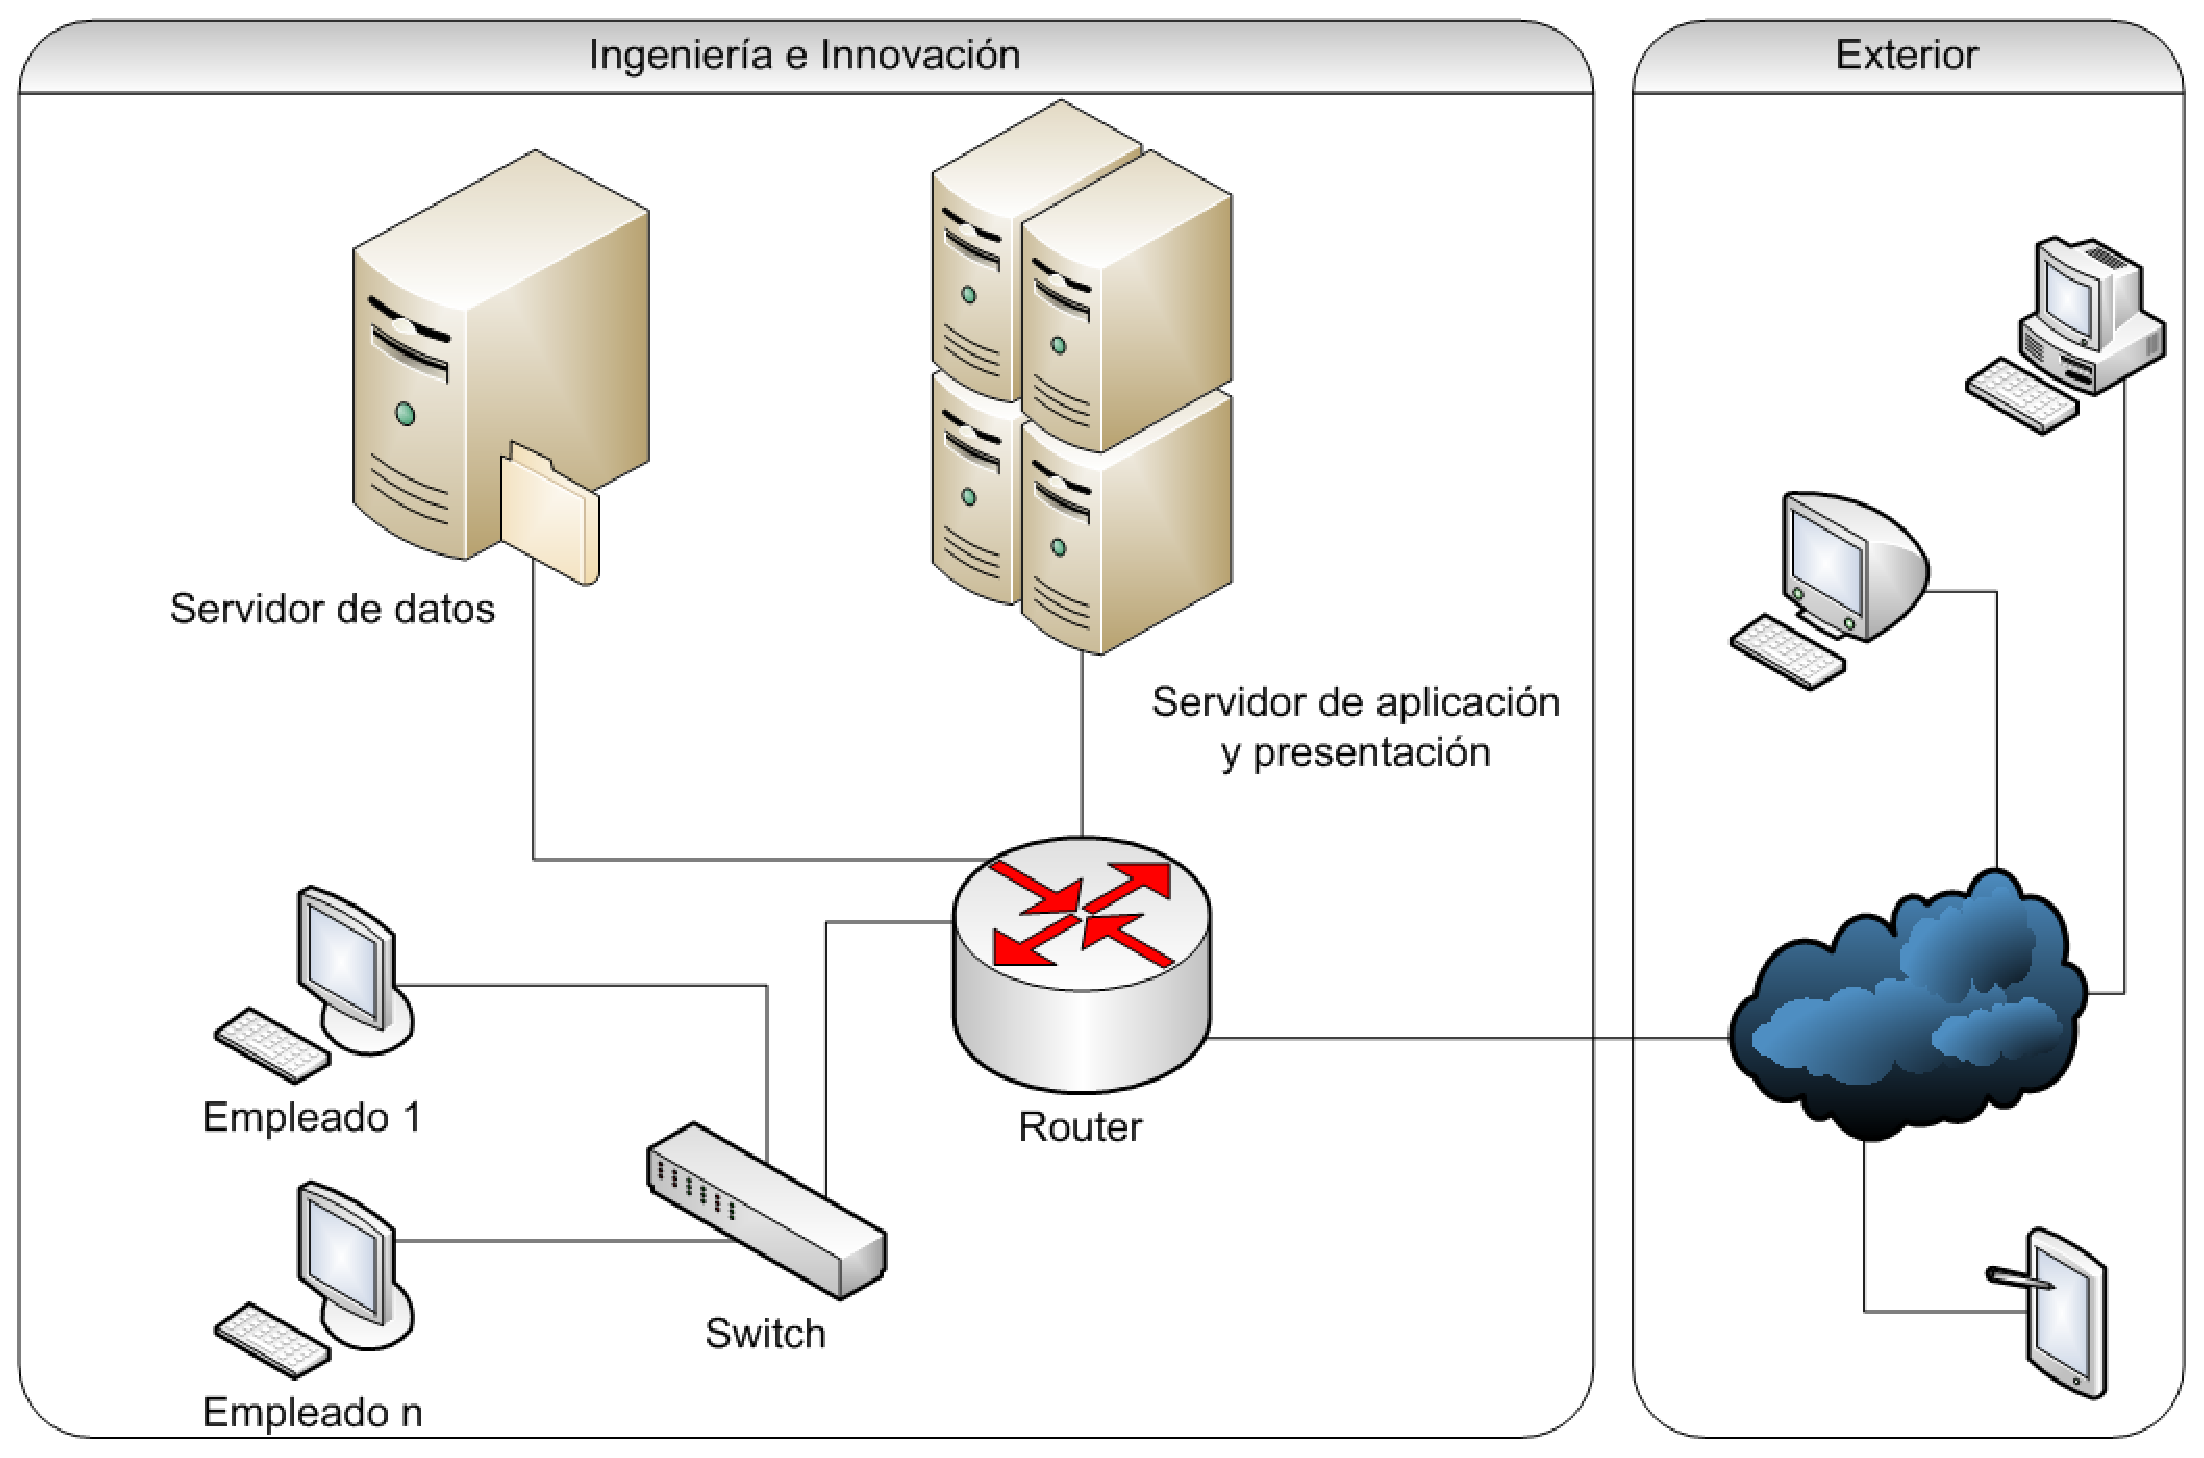
\epsfig{file=imagenes/arquitectura_iandi,width=5.28in}
\caption{Arquitectura hardware de la empresa.}
\label{fig:arquitectura_iandi}
\end{figure}

En el plano de la programación, y a pesar de que PHP ofrece el paradigma de
orientación a objetos desde su versión 3 (Junio de 1998), se ha optado por
seguir con el paradigma imperativo presente en el resto de la aplicación.

\subsection{Alternativas de implementación}

Las alternativas a la implementación son numerosas, pero ninguna de ellas
resultaba razonable dadas las características descritas en los párrafos
anteriores:

\begin{itemize}
\item Podrían haberse empleado otros lenguajes de programación del lado del
servidor, desde Perl, Python, Ruby... e incluso la tecnología ASP, aunque
en este último caso debería haberse pasado a usar IIS como servidor web;

\item Comprendiendo las ventajas que ofrece la programación orientada a objetos,
el proyectante se planteó realizar los nuevos módulos usando este paradigma,
pero la posibilidad se descartó debido a la fuerte dependencia del sistema con
conceptos previamente tratados de forma imperativa. Un cambio en este sentido
habría supuesto la convivencia de dos modelos diferenciados o la definición de
clases para el tratamiento de unos objetos que si bien interactúan con la nueva
funcionalidad, no forman parte del marco de desarrollo de este proyecto.
\end{itemize}

Además, una vez que el proyectante finalizase su labor en la empresa, el sistema
sería mantenido por ingenieros industriales con conocimientos de PHP pero sin
la formación básica de orientación a objetos.

\section{Hechos relevantes y asunciones}

\subsection{Hechos}

\begin{itemize}
 \item La interfaz será desarrollada siguiendo las especificaciones HTML 4.01 y
CSS2, ya que es la manera en que está desarrollado el resto de la aplicación,
sin perjuicio de incluir puntualmente funcionalidades de HTML5 y CSS3.
\item La aplicación estará instalada en un servidor de Ingeniería e Innovación
\item Debe estar disponible 24 horas al día, 7 días a la semana.
\end{itemize}

Un hecho que merece mención aparte es que el proyecto no es independiente, es
decir, forma parte de un sistema mayor en uso. De esta manera, es necesario que
se adapte de la forma más \textit{suave} posible a aquel sistema. Para ello, se
estudió en profundidad su funcionamiento y se adoptaron todas las convenciones
que fue posible, desde la forma que el sistema existente tenía de almacenar
fechas en la base de datos, hasta los métodos para comprobar en cada página que
un usuario está autenticado.

\subsection{Asunciones}

\begin{itemize}
\item El usuario usa un ordenador de escritorio con un navegador web. Otros
dispositivos (p. ej.:móviles) no están soportados.
\item El usuario no tiene problemas graves de accesibilidad. El desarrollo no
se centrará en la accesibilidad del producto más allá de seguir las
recomendaciones de las especificaciones HTML 4.01 y CSS2.
\item En general, la herramienta se utilizará de manera local en las
instalaciones del cliente, pero el portal web permite acceso a la intranet
desde el exterior (extranet), por lo que el rendimiento de la herramienta debe
estar adaptado a esta característica.
\end{itemize}

\section{Aspectos relativos a los usuarios dentro del sistema}
\label{sec:usuarios_del_sistema}

La aplicación, tal y como se encontraba al inicio de este proyecto, contaba con
dos tipos de usuarios: usuario básico y Administrador.

\subsection{Usuario básico}
\label{sec:usuario_basico}

Todos los miembros de la empresa tienen un usuario creado en la base de datos
que les permite gestionar temas relativos a proyectos, expedientes,
facturación... La información es común a todos los miembros de la organización,
y el único control que se lleva a cabo es el registro de cuándo y quién realizó
la última actualización de los datos. La organización es los suficientemente
pequeña para que este sistema haya permitido durante al menos dos años de
existencia de la aplicación, una gestión más ágil sin provocar errores o
inconsistencias notables.

\subsection{Administrador}
\label{sec:administrador}

El Administrador puede dar de alta/baja usuarios y realizar operaciones
delicadas relativas a la modificación de datos considerados estáticos (no
deberían cambiar a lo largo del tiempo, pero pueden haberse introducido
erróneamente), y al borrado de datos de la base de datos, que siempre ha de
meditarse y valorarse detenidamente.

En los nuevos módulos desarrollados por el proyectante se ha mantenido la
misma metodología. Si bien se planteó la posibilidad de que el acceso a
determinados datos (facturas, proyectos, etc.), solamente estuviera autorizado
según qué usuario intentase acceder, esta posibilidad se desestimó, de nuevo,
debido al pequeño tamaño de la organización y al buen resultado que ha tenido un
sistema más abierto.

También se planteó la posibilidad de abrir la aplicación a los clientes
externos, de manera que ellos mismos pudieran introducir los datos de horas
trabajadas por sus empleados en lugar de tener que proporcionar esa información
a Ingeniería e Innovación y que fuera un empleado de ésta última quien
finalmente grabase los datos. Este sistema ahorraría un paso en el proceso y
los errores que se pudieran derivar de ello; sin embargo, y por motivos de
seguridad, se decidió que la apertura de la aplicación se aplazaría hasta
futuros ciclos de desarrollo.